\documentclass[10pt,a4paper,twocolumn,twoside,UTF8]{ctexart}
\usepackage{geometry}
	\geometry{left=2cm,right=2cm,top=2.5cm,bottom=3cm}
\usepackage{xeCJK,amsmath,paralist,enumerate,booktabs,multirow,graphicx,subfig,setspace,listings}
	\setlength{\parindent}{2em}%正文首行缩进两个汉字
	\lstset{language=tex}
\usepackage{titlesec}
	\newfontfamily\sectionef{Times New Roman}
	\setCJKfamilyfont{FZHeiTi}{黑体}
	\newcommand{\sectioncf}{\CJKfamily{FZHeiTi}}
	\titleformat*{\section}{\large\bfseries\sectioncf\sectionef}
	\titleformat*{\subsection}{\normalsize\bfseries\sectioncf\sectionef}
\usepackage{fancyhdr}
\usepackage{layout}
\setlength\columnsep{0.8cm}%设置双栏的间距


%%begin----------设置首页和正文不同的页眉页脚----------------%%

\usepackage{ifthen}%这个宏包提供逻辑判断命令
\newboolean{first}%引入布尔变量
\setboolean{first}{true}%将布尔变量设置为true
\pagestyle{fancy}

	\fancypagestyle{maincontent}{
		\fancyhf{}  %清空页眉页脚设置
		\fancyhead[EL, OR]{\thepage}
		\fancyhead[EC]{实验B12 温度测控仪的设计与组装}
		\fancyhead[OC]{基\quad 础\quad 物\quad 理\quad 实\quad 验}
		\renewcommand\headrulewidth{0pt}
	}

	%%% Step2 定义首页的页面风格
	%页眉中间的双行文字,大小和字间距需要微调
	%左右的内容是年月,可以自己修改寻找自动获取的方法
	\usepackage{datetime}
		%\shortmonthname可以获取英文月份缩写
	\fancypagestyle{firstpage}{
		\setboolean{first}{false}%firstpage出现,则将first重置为false
		\fancyhf{}  %清空页眉页脚设置
		\fancyhead[L]{\the\year 年\the\month 月}
		\fancyhead[R]{\shortmonthname[\the\month], \the\year}
		\fancyhead[C]{
		\large{基\quad 础\quad 物\quad 理\quad 实\quad 验}\\
		\normalsize{GENERAL PHYSICS LABORATORY}
		}
	}

	%%% Step3 页眉线的设置:用布尔变量区分首页和正文
	\newcommand{\makefirstpageheadrule}{%定义首页页眉线-双线绘制命令
	\makebox[0pt][s]{\rule[0.6\baselineskip]{\headwidth}{0.3pt}}
	\makebox[0pt][s]{\protect\hspace{-0.34em}\rule[0.75\baselineskip]{\headwidth}{0.3pt}}
	\protect\vspace{-20pt}
	%\rule[9pt]{\headwidth}{0.3pt}
	% \rule[25pt]{\headwidth}{0.3pt}
	%\rule[raise-height]{width}{height}
	%其中第一个可选参数为将直线抬多高
	}

	\newcommand{\makeheadrule}{%定义正文页页眉线绘制命令,单线
	\makebox[0pt][l]{\rule[1\baselineskip]{\headwidth}{0.3pt}}
	\protect\vspace{-20pt}%页眉和正文的距离
	}

	%根据布尔变量first为true或false分别执行不同的页眉线绘制命令
	\renewcommand{\headrule}{%重定义headrule命令
	\ifthenelse{\boolean{first}}{\makeheadrule}
	{\makefirstpageheadrule}
	}


%%end--------------设置首页和正文不同的页眉页脚-----------%%



%%begin-----------------参考文献-----------------------%%

\usepackage[colorlinks,linkcolor=blue,urlcolor=blue]{hyperref}%超链接
\usepackage[hyperref=true,backend=biber,bibstyle=gb7714-2015,citestyle=numeric-comp,sorting=none,backref=true]{biblatex}
	%hyperref=true和backref=true表示为各个参考文献的引用处、及定理、定义、例子等的引用处都添加上超链接;
	%backend=biber:后端处理的程序为biber.exe
	%bibstyle:参考文献风格;每个期刊、组织要求不同
		%gb7714-2015是目前国内期刊通用的风格,称为gb标准风格
	%citestyle:引用风格;每个期刊、组织要求不同
	%sorting=none:按照参考文献在论文中出现的先后顺序排序。
	%**编译:biblatex与biber命令配合使用。xelatex-biber-xelatex-xelatex
\addbibresource{book.bib}
	%这里写上.bib文件的相对地址
	%每次实验引用的页数不同,需要手动改变

%%end-------------------参考文献-----------------------%%





%%%%%%%%%%%%%%%%%%%%%%%%%%%%%%%%%%%%%%%%%%%%%%%%%%%%%%%%%%
%%%%%%%%%%%%%%%%%%%%%%%%%正文开始%%%%%%%%%%%%%%%%%%%%%%%%%%
%%%%%%%%%%%%%%%%%%%%%%%%%%%%%%%%%%%%%%%%%%%%%%%%%%%%%%%%%%

\begin{document}


%%begin-------------------中文摘要-----------------------%%
\title{\LARGE\textbf{用交流电桥测电感电容}\footnotemark[1]}
\author{\large\textit{XXX xxxxxxxx}$^{1}$\footnotemark[2]
\\ \normalsize{(1 \textit{中山大学 物理学院,广东 广州 }510275)}}
\date{}%不显示日期

\twocolumn[
	%twocolumn: 双栏article下的单栏摘要
	\begin{@twocolumnfalse}
	\maketitle  %标题和作者
  	\renewcommand{\abstractname} {} %不显示摘要名字
	\begin{abstract}
	\vspace{-3em}
	%vspace:调整垂直空白,可以自己调整;缩小abstract和center(以及maketitle)的间距
	%\noindent %备用:摘要无缩进
	{\bf 摘{} 要:}
	{\small 本次实验以电桥的平衡条件为基本, 测量了电容器的电容量, 损耗电阻以及电感器的电感量和品质因数。
	用 NI VirtualBench-8012 一体化仪器及成品数字电桥测量相同参数并与其进行对比, 最后测量未知四端网络的连线方式及元件参数。 根
	据实验搭建的电路测得电容 $C_x=46.7nF$,损耗电阻 $r_c=51.5 \Omega $, 损耗因数$D=0.0024$, 电感 $L_x=14.8mH$, 电阻 $r_L=61.7\Omega$, 品质因数$Q=0.24$。
	用数字电桥测得电容 $C_x=47.1nF$,损耗电阻 $r_c= 51.5\Omega $, 损耗因数$D=0.0024$, 电感 $L_x=20.2mH$, 电阻 $r_L=135\Omega$, 品质因数$Q=0.15$。
	另外, 利用实验室的仪器, 测得了12号黑盒中不同接口的电路情况, 推测出了黑盒内部的电路。
	最后利用 Multisim 电路仿真软件以 RLC 串联电路实验为例进行仿真模拟。
	RLC 电路测出的谐振频率为1584.9Hz,由实验B5测得谐振点频率为1342.54Hz,仿真结果与其相对误差为18.05\%
	。非平衡直流电桥实验与理论值几乎吻合, 交流电桥测电容和电感的实验中, 交换元件前后结果没有改变。}
	\par%空的新行的高度。
	\textbf{关键词}:交流电桥; 电感; 电容; 数字电桥; Multisim 电路仿真软件; RLC 串联电路; 非平衡直流电桥; 交流电桥测电容和电感
	\vspace{2em}
	\end{abstract}
	\end{@twocolumnfalse}
]
\renewcommand{\thefootnote}{\fnsymbol{footnote}}
\footnotetext[1]{由中山大学物理学院陆佑堂提供器材和指导。}
\footnotetext[2]{通信作者,\url{xxxx@mail2.sysu.edu.cn}}
%%end-------------------中文摘要-----------------------%%


\thispagestyle{firstpage}%首页页面风格:firstpage
\pagestyle{maincontent}%第二页之后的页面风格:maincontent


%%begin----------------层级结构------------------------%%

%重点1:知道每一个层级的样式和怎么和后面的正文接上
%重点2:掌握各种换段的方法
%重点3:自定义的项目符号(宏包enumerate的用法)

\section{引 \quad 言}
	%%section:第一级,节	,1
	交流电桥可较精确地测量电容器的电容量、 自感系数、 互感系数及线圈的品质因数等, 用途广泛。
	本实验将介绍用交流电桥测量电容和电感的基本原理及测量方法, 测量电容器的电容、 损耗电阻和损耗因数,
	测量电感器的电感、 电阻和品质因数。
		%%section后面的正文:自动换段,正常缩进
	%%引用参考文献语法\cite{},标识符shenhan2015被称为citekey,可以在book.bib文件中找到,是@后面的一串文字。论文最后的参考文献只会打印行文过程中cite的文献,而不是book.bib文件中的所有文件。
%自然换段有两种方式, 一种是使用命令\lstinline|\par|, 另一种是常用的直接空一行即可.
	%%自然换段:\par;相当于空一行,见下面的193行
	在电路仿真软件中,NI Multisim 软件是一个专门用于电子电路仿真与设计的 EDA 工具软件。 作为 Windows 下
	运行的个人桌面电子设计工具, NI Multisim 是一个完整的集成化设计环境,利用
	计算机仿真与虚拟仪器技术可以很好地解决理论教学与实际动手实验相脱节的这一问题。
	Multisim 具有直观的图形界面、 丰富的元器件、 强大的仿真能力和丰富的测试仪器, 是电
	子学教学的首选软件工具。%下面将换栏!换栏不同于换页。换栏我们使用命令\lstinline|\newpage|, 而换页我们用命令\lstinline|\clearpage|.
\newpage
%换一栏,而不是换一页。换一页用\clearpage

\section{介\quad 绍}
%在论文写作中, 我们通常用到的\LaTeX 中的层级结构如下, 包括会进入pdf目录的章节结构\lstinline|\section|, \lstinline|\subsection|, \lstinline|\subsubsection|和不会进入目录的段落结构\lstinline|\paragraph|, \lstinline|\subparagraph|.
    \subsection{RLC串联电路}
    RLC 串联电路如图1(a)所示,有
	\begin{equation}
		U=U_R+U_L+U_C=I[R+j \omega L+\frac{1}{j\omega C}]
	\end{equation}
    可得总阻抗的模$|ܼZ|$、 电流有效值I、电路电流与总电压之间的相位差$\varDelta \varphi$ 分别为
    \begin{equation}
		|Z|=\sqrt{R^2+\left(\omega L-\frac{1}{\omega C}\right)^2}
	\end{equation}

    \begin{equation}
		I=\frac{U}{\sqrt{R^2+\left(\omega L-\frac{1}{\omega C}\right)^2}}
	\end{equation}

	\begin{equation}
		U_R=IR=\frac{UR}{\sqrt{R^2+\left(\omega L-\frac{1}{\omega C}\right)^2}}
	\end{equation}

	\begin{equation}
		\varDelta \varphi=\varphi_{U_R}-\varphi_U=-arctan\left(\frac{\omega L-\frac{1}{\omega C}}{R}\right)
	\end{equation}

    若总电压有效值ܷ保持不变, 根据式(3)、(5)可画出݂$I-f$幅频特性曲线和$\varDelta\varphi- f$相频特性曲线, 分别如图 1(b) 和(c)所示。
    定义参数
    \begin{equation}
		Q=\frac{U_0}{U}=\frac{1}{R\omega_0 C}=\frac{\omega_0 I}{R}
	\end{equation}
    该参数称为谐振电路的品质因数, 简称Qܳ值, 是表征谐振电路性能优劣的重要物理量之一。
	谐振时,$U_C=U_L=QU$,所以ܳQ值越大, 电感、 电容上的电压与总电压的比值也越大, 电路储能效率越高。

	\begin{figure}[htbp]
		\centering
		\subfloat[测量电路]{\label{fig:RLCa}
		\includegraphics[width=0.16\textwidth]{img/1a.png}%调节这里的图片宽度
		}%
		\subfloat[幅频特性]{\label{fig:RLCb}
		\includegraphics[width=0.16\textwidth]{img/1b.png}%调节这里的图片宽度
		}%
		\subfloat[相频特性]{\label{fig:RLCc}
		\includegraphics[width=0.16\textwidth]{img/1c.png}%调节这里的图片宽度
		}%
		\caption{RLC串联电路的稳态特性}
		\label{fig:RLC}
	\end{figure}
\subsection{交流电桥及其平衡条件}
		%%subsection:第二级,小节,2.1
		交流电桥的原理如图2(a)所示,$Z_1$、$Z_2$、$Z_3$、$Z_4$分别为四个桥臂的复阻抗。 调节各臂的阻抗, 使电桥达
		到平衡, 即 A 和 B 两点间的电位差为零, 则有ܼ$\frac{Z_1}{Z_2}=\frac{Z_3}{Z_4}$, 即交流电桥相对两臂交
		流阻抗的乘积相等, 此即为交流电桥的平衡条件。 用复数形式表示为$\frac{|Z_1|e^{i \varphi_1}}{|Z_2|e^{i \varphi_2}}=\frac{|Z_3|e^{i \varphi_3}}{|Z_4|e^{i \varphi_4}}$,
		相当于$\frac{|Z_1|}{|Z_2|}=\frac{|Z_3|}{|Z_4|}$和$\varphi_1-\varphi_2=\varphi_3-\varphi_4$同时成立。
		可见, 交流电桥平衡时, 除相对两臂交流阻抗的模的乘积相等外, 阻抗相对两臂
		相位角的和值相等, 这是它和直流电桥的主要差别。 为使电桥平衡, 要依照上式配置各桥臂的阻抗。 在电
		桥平衡过程中要反复调节这些参数。		%%subsection后面的正文:自动换段,正常缩进
	
		\subsection{测量电容器的电容C及其损耗因素D}
		%%subsubsection: 第三级,小小节,2.1.1
		实际电容不是理想的电容器, 在电路中会损耗能量, 故其等效电路可看成是一个纯电容$C_x$和一个损耗
		电阻$r_c$的串联或并联电路, 本实验将采用串联等效电路来处理。 由于存在损耗, 当正弦信号通过它时, 电
		容器两端的电压与通过电容器的电流之间的相位差$\varphi$不是$90^{\circ}$ , 而是$\varphi=90^{\circ}-\delta$ 其中$\delta$称为电容器的损
		耗角, 它的正切值称为电容器的损耗因数, 表示为D。 它随损耗电阻$r_c$的增加而变大, 是衡量电容器质
		量优劣的一个重要参数, 可写为$D=tan\delta=r_c \omega C_x$.
		电容电桥适合测量损耗较小的电容, 测量电路如图 2(b) 所示,$R_2$和$R_4$耗为纯电阻,$C_0$为标准电容, 它的损
		耗电阻$R_C$在低频时近似为零。 为了相平衡,$C_0$串联了一个电阻$R_0$。 根据电桥各臂配置的情况可得$C_x=\frac{C_0 R_2}{R_4}$,$r_c=\frac{R_0 R_2}{R_4}$ ,$D=\omega R_0 C_0$为了调节方便, 实验过程中常固定$R_0$和$R_2$的数值, 直到交流
		电桥 AB 点间的电压 AB 最小。

				%%subsubsection后面的正文:自动换段,正常缩进
				\begin{figure}[htbp]
					\centering
					\subfloat[交流电桥原理]{\label{fig:2a}
					\includegraphics[width=0.16\textwidth]{img/2a.jpg}%调节这里的图片宽度
					}%
					\subfloat[电容电桥]{\label{fig:2b}
					\includegraphics[width=0.16\textwidth]{img/2b.jpg}%调节这里的图片宽度
					}%
					\subfloat[麦克斯韦尔-维恩电桥]{\label{fig:2c}
					\includegraphics[width=0.16\textwidth]{img/2c.jpg}%调节这里的图片宽度
					}%
					\caption{不同类型的电桥}
					\label{fig:2}
				\end{figure}

		\subsection{测量电容器的电感量L及其品质因素Q}
	由于任何电感线圈都具有损耗电阻, 故其等效电路可看作是一个纯电感L和损耗电阻$r_L$的串联。 实际
	使用过程中常希望$r_L$尽可能小, 以减小能量的损耗。 $r_L$越小, 电感的品质因数ܳ$Q=\frac{\omega L_x}{r_L}=\omega R_0 C_0$越大。 品质因数
	ܳ是衡量电感线圈质量好坏的一个重要参数。
	如图2(c)麦克思威尔-维恩电桥是一种最常用的测量电感的电桥。 参照电容电桥的分析方法,
	可得电感电桥平衡时有$L_x=C_0 R_2 R_3=\frac{R_2 R_3}{R_0}=\frac{\omega L_x}{r_L}=\omega R_0 C_0$,其中$R_0$和$R_2$为独立变量, 反复交
	替调节可使电桥趋于平衡。

	\section{实验步骤}
	\subsection{基于Multisim电路仿真软件的RLC串联电路特性}
	\subparagraph{步骤一}基于Multisim电路仿真软件的RLC串联电路如图3所示。电路中电阻、电感和电容参
	数分别为1000Ω,20mH, $0.47\mu F$。
	\subparagraph{步骤二}参照实验B5,自拟数据记录表格,测量RLC电路的幅频和相频特性,并将模拟结果与上学期完成的实验结果进行对比。
	
	\begin{figure}[!h]
		\centering
		\includegraphics[width=0.4\textwidth]{img//RLC.jpg}
			%textwidth:正文宽度。双栏,则将两栏正文宽度相加。
		\caption{RLC串联电路}
		\label{fig:3}
	\end{figure}

	\subsection{测量电容器的电容量及其损耗因素D}
    \subparagraph{步骤一}按图 2(b) 连接线路,要求桥臂接线尽可能短且接触良好。$R_0$和$R_4$采用电阻箱作为可调节参数,
固定$C_0$和$R_2$的数值不变。
    \subparagraph{步骤二}调节$R_0$使$U_{AB}$为极小值,再调节$R_4$使$U_{AB}$更小,交替调节若干次,直至$U_{AB}$值最小为止,
此时不论调节$R_0$还是$R_4$都会使$U_{AB}$值增大。由于判断$U_{AB}$最小值时人为误差较大,需进行多次测量。
    \subparagraph{步骤三}将$R_4$和$R_0$被测电容互换位置,用相同方法调节电桥平衡并记录多组$R_0$和$R_4$的数值。
    \subparagraph{步骤四}计算待测电容的$C_x$、$r_c$和D的数值及实验标准差。

    \subsection{测量电感器的电感量及品质因数}
    \subparagraph{步骤一}采用如图2(c)所示的电路,固定$R_3$和$C_0$的数值,$R_0$和$R_2$采用电阻箱,反复调节$R_0$和$R_2$的数值直至
$U_{AB}$数值最小,电桥平衡。
\subparagraph{步骤二}记录相关数据并计算待测电感的$L_x$、$r_L$和Q的数值及实验标准差。测量过
程中需类似实验内容2的方法进行“换臂”测量,以减小系统误差。
    
    \subsection{用成品数字电桥测电容和电感}
	\subparagraph{步骤一}采用数字电桥测量上述待测电容和电感的相关参数,并与实验内容2和3的结果进行比较。

	\subsection{测量未知四端网络的连线方式及元件参数}
	\subparagraph{步骤一}由教师指定一个测试盒,盒内为 1~3 个基本元器件( R、L、C)的串联或并联电路,每
种元件最多只有一个,或者没有。测试盒不透明,实验者看不见内部电路。
    \subparagraph{步骤二}每个测试盒表面有编号,盒外有四个接线柱,要求实验者综合利用已学交直流电路知识和
设备,自行选择合适的仪器,自行设计测量方法,确定盒内电路的形式及各元件的参数。要求画出
盒内的电路,并标出元件参数。

    \subsection{利用Multisim软件仿真直流电桥和交流电桥实验 }
    \subparagraph{仿真交流电桥测电容实验} 

	电路如图4)所示。其中电阻$R_1 = 51\Omega$,$R_2 = 510\Omega$,可调电阻 $R_3 = 100\Omega$, 可调
	电阻 $R_4 = 1k\Omega$,电容$C_1 = 0.1\mu F$ , $C_2 = 0. 47\mu F$ ,信号为正弦信号,频率为10kHz,
	电压幅峰值 $V_{PP} = 5V$。测完后“换臂”(图右)再测。
	\begin{figure}[!h]
		\centering
		\includegraphics[width=0.44\textwidth]{img//4.jpg}%调节这里的图片宽度
		\caption{仿真交流电桥测电容实验}
		\label{fig:4}
	\end{figure}

	\subparagraph{仿真交流电桥测电感实验} 

	电路如图5(a)、5(b)所示。其中电阻$R_1 = 100\Omega $,$R_3 = 510\Omega$,可调电阻 $R_2 = 1k\Omega$, 可调
电阻 $R_4 = 1k\Omega$,电容$L_1 = 20mH $, $C_1 = 0.47\mu F$ ,信号为正弦信号,频率为10kHz,
电压峰峰值 $V_{PP} = 5V$。测完后“换臂”再测。

\begin{figure}[!h]
	\centering
	\subfloat[换臂前]{\label{fig:5a}
	\includegraphics[width=0.22\textwidth]{img//5a.jpg}%调节这里的图片宽度
	}%
	\subfloat[换臂后]{\label{fig:5b}
	\includegraphics[width=0.22\textwidth]{img//5b.jpg}%调节这里的图片宽度
	}%
	\caption{仿真交流电桥测电感实验}
	\label{fig:5}
\end{figure}

    \subsection{实验结果分析}
将自组交流电桥测量结果、Multisim 仿真结果和成品数字电桥测量结果三者进行比较。


\section{实验数据分析}

\subsection{基于Multisim电路仿真软件的RLC串联电路特性}
电路中电阻、电感和电容参数分别为1000Ω,20mH,$0.47\mu F$。

作RLC串联电路的幅频和相频特性曲线,如图6,7:

\begin{figure}[!h]
	\centering
	\includegraphics[width=0.45\textwidth]{img//6a.png}%调节这里的图片宽度
	\caption{幅频特性曲线}
	\label{fig:6}
\end{figure}

\begin{figure}
	\centering
	\includegraphics[width=0.45\textwidth]{img//6b.png}%调节这里的图片宽度
	\caption{相频特性曲线}
	\label{fig:7}
\end{figure}

图中谐振点频率为1584.9Hz,由实验B5测得谐振点频率为1342.54Hz,仿真结果与其相对误差为18.05\%.
实验误差主要在于实验B5取样点太少,拟合后相频曲线不光滑,不能很好反映电路的相频特性,故谐振点的读数会有所偏差。

\subsection{测量电容器的电容量及其损耗因素}
电路中$C_0=0.47\mu F$,$R_0=510\Omega$,交流电频率$f=1kHz$,$U=10V$。
\begin{table}[!h]
	\centering
	  \begin{tabular}{c|cccc}
	  \toprule
	  \multicolumn{1}{c}{} & 实验次数  & $R_2/\Omega $   & $R_4/\Omega$   & $U_{AB}/mV$  \\
	  \midrule
	  \multicolumn{1}{c}{\multirow{5}[2]{*}{换臂前}} & 1     & 10.6 & 108.4  & 0.101  \\
	  \multicolumn{1}{c}{} & 2     & 10.8 & 108.6  & 0.118 \\
	  \multicolumn{1}{c}{} & 3     & 10.8 & 108.7  & 0.108 \\
	  \multicolumn{1}{c}{} & 4     & 10.8 & 108.5  & 0.116  \\
	  \multicolumn{1}{c}{} & 5     & 10.8 & 108.3  & 0.108  \\
	  \midrule
	  \multicolumn{1}{c}{}  & 平均值:  & 10.8 & 108.5 & \\
	  \multicolumn{1}{c}{}& 标准差:  & 0.0 & 0.1 &  \\
	  \midrule
	  \multicolumn{1}{c}{\multirow{5}[2]{*}{换臂后}} & 1     & 11.2 & 113.0  & 8.134\\
	  \multicolumn{1}{c}{} & 2     & 11.2 & 113.1  & 7.939 \\
	  \multicolumn{1}{c}{} & 3     & 11.2 & 113.4 & 5.981 \\
	  \multicolumn{1}{c}{} & 4     & 11.2 & 113.7 & 8.192\\
	  \multicolumn{1}{c}{} & 5     & 11.2 & 113.5 & 7.989 \\
	  \midrule
	  \multicolumn{1}{c}{}& 平均值:  & 11.2 & 113.4 &  \\
	  \multicolumn{1}{c}{}& 标准差:  & 0.0 & 0.3 &  \\
	  \bottomrule
	  \end{tabular}%
   \caption{交流电桥测电容数据}	  
   \label{tab:1}
  \end{table}%

  换臂前数据计算
  \[\left\{%\left和\right配合使用,可以得到大小匹配的各种括号
  \begin{aligned}
  &C_x=\frac{C_0 R_2}{R_4}=46.9 nF\\
  &r_c=\frac{R_0 R_2}{R_4}=52.5\Omega\\
  &D=\omega r_c C_x=0.0025
  \end{aligned}
 \right.
\]

换臂后数据计算
\[\left\{%\left和\right配合使用,可以得到大小匹配的各种括号
\begin{aligned}
&C_x=\frac{C_0 R_2}{R_4}=46.4\mu F\\
&r_c=\frac{R_0 R_2}{R_4}=50.4\Omega\\
&D=\omega r_c C_x=0.0023
\end{aligned}
\right.
\]

对换臂前后的数据取均值后计算,如表2所示:
\begin{table}[!h]
	\centering
	  \begin{tabular}{cccc}
	  \toprule
	     & 实验测量 & 成品电桥测量 & 相对误差/\% \\
	  \midrule
	  $C_x/nF$   & 46.7   & 94.8   & 103.0 \\
	  $r_c/\Omega$  & 51.5   & 52.5   & 1.9 \\
	  D  & 0.0024   & 0.0050   & 116.6 \\
	  \bottomrule
	  \end{tabular}%
	\caption{实验测量值与成品电桥测量值对比表}
	\label{tab:2}%
  \end{table}%

  仿真结果见表3:
  电路中$C_0=0.47\mu F$,$R_0=510\Omega$,交流电频率$f=1kHz$,$U=10V$。
  \begin{table}[!h]
	\centering
	  \begin{tabular}{cccc}
	  \toprule
	     & 换臂前 & 换臂后 & 平均值 \\
	  \midrule
	  $R_2\Omega$ & 10.9 &11 & \\
	  $R_4\Omega$ & 108.8 &110&\\
	  $C_x/nF$   & 47.1   & 47   & 47.1 \\
	  $r_c/\Omega$  &  51.1  & 51  & 51.1 \\
	  \bottomrule
	  \end{tabular}%
	\caption{仿真交流电桥测电容实验数据}
	\label{tab:3}%
  \end{table}%

由公式得仿真电路得电感品质因素D:
\begin{equation*}
	D=\omega r_c C_x=0.0024
\end{equation*}

将实验测量值与仿真结果比较,结果见表4:
\begin{table}[!h]
	\centering
	  \begin{tabular}{cccc}
	  \toprule
	     & 实验测量 & 仿真测量 & 相对误差/\% \\
	  \midrule
	  $C_x/nF$   & 46.7   & 47.1   & 0.9 \\
	  $r_c/\Omega$  & 51.5   & 51.1   & 0.8 \\
	  D  & 0.0024   & 0.0024   & 0 \\
	  \bottomrule
	  \end{tabular}%
	\caption{实验测量值与仿真值对比表}
	\label{tab:4}%
  \end{table}%


\subsection{测量电感器的电感量及品质因数}
电路中$C_0=0.47\mu F$,$R_0=510\Omega$,交流电频率$f=1kHz$,$U=10V$。
\begin{table}[!h]
	\centering
	  \begin{tabular}{c|cccc}
	  \toprule
	  \multicolumn{1}{c}{} & 实验次数  & $R_2/\Omega$   & $R_3/\Omega$   & $U_{AB}/mV$  \\
	  \midrule
	  \multicolumn{1}{c}{\multirow{5}[2]{*}{换臂前}} & 1     & 81.9 & 358.3  & 4.411  \\
	  \multicolumn{1}{c}{} & 2     & 92.0 & 361.1  & 2.580 \\
	  \multicolumn{1}{c}{} & 3     & 92.0 & 361.2  & 2.580 \\
	  \multicolumn{1}{c}{} & 4     & 91.0 & 361.2  & 2.613  \\
	  \multicolumn{1}{c}{} & 5     & 92.0 & 361.0  & 2.579  \\
	  \midrule
	  \multicolumn{1}{c}{}  & 平均值:  & 89.8 & 360.5 &  \\
	  \multicolumn{1}{c}{}  & 标准差:  & 3.9 & 1.1 &  \\
	  \midrule
	  \multicolumn{1}{c}{\multirow{5}[2]{*}{换臂后}} & 1     & 87.6 & 349.1  & 4.958\\
	  \multicolumn{1}{c}{} & 2     & 87.5 & 349.1  & 4.832 \\
	  \multicolumn{1}{c}{} & 3     & 87.5 & 349.0  & 4.807 \\
	  \multicolumn{1}{c}{} & 4     & 87.5 & 348.9  & 4.782\\
	  \multicolumn{1}{c}{} & 5     & 87.5 & 348.8  & 4.760 \\
	  \midrule
	  \multicolumn{1}{c}{}& 平均值:  & 87.5 & 349.0 &  \\
	  \multicolumn{1}{c}{}& 标准差:  & 0.0 & 0.1 &  \\
	  \bottomrule
	  \end{tabular}%
   \caption{交流电桥测电感数据}
   \label{tab:5}
  \end{table}%

  换臂前数据计算
  \[\left\{%\left和\right配合使用,可以得到大小匹配的各种括号
  \begin{aligned}
  &L_x=C_0 R_2 R_3=15.2 mH\\
  &r_L=\frac{R_2 R_3}{R_0}=63.5\Omega\\
  &Q=\frac{\omega L_x}{r_L}=0.24
  \end{aligned}
 \right.
\]

换臂后数据计算
\[\left\{%\left和\right配合使用,可以得到大小匹配的各种括号
\begin{aligned}
&L_x=C_0 R_2 R_3=14.4 mH\\
&r_L=\frac{R_2 R_3}{R_0}=59.9\Omega\\
&Q=\frac{\omega L_x}{r_L}=0.24
\end{aligned}
\right.
\]

对换臂前后的数据取均值后计算,如表6所示:
\begin{table}[!h]
	\centering
	  \begin{tabular}{cccc}
	  \toprule
	     & 实验测量 & 成品电桥测量 & 相对误差/\% \\
	  \midrule
	  $L_x/mH$   & 14.8  & 20.2   & 36.5 \\
	  $r_L/\Omega$  & 61.7   & 135.0   & 118.8 \\
	  Q  & 0.24   & 0.15   & 37.5 \\
	  \bottomrule
	  \end{tabular}%
	\caption{实验测量值与成品电桥测量值对比表}
	\label{tab:6}%
  \end{table}%

仿真实验中,$L_x=20 mH$,$r_L=100\Omega$,
由公式得仿真电路得电感品质因素D:
\begin{equation*}
	Q=\frac{\omega L_x}{r_L}=0.2
\end{equation*}

将实验测量值与仿真结果比较,结果见表7:
\begin{table}[!h]
	\centering
	  \begin{tabular}{cccc}
	  \toprule
	     & 实验测量 & 仿真测量 & 相对误差/\% \\
	  \midrule
	  $L_x/mH$   & 14.8  & 20.0   & 35.1 \\
	  $r_L/\Omega$  & 61.7   & 100.0  & 62.1 \\
	  Q  & 0.24   & 0.2   & 16.7 \\
	  \bottomrule
	  \end{tabular}%
	\caption{实验测量值与仿真测量值对比表}
	\label{tab:7}%
  \end{table}%




  由上述数据可知, 不论与成品数字电桥的测量结果还是与 Multisim 仿真结果相比, 实验结果的相对误
差都较大。 但相比于使用成品数字电桥测得的结果, 实验测得的结果与 Multisim 仿真结果的误差更小。 原
因可能有以下几点:
\begin{enumerate}
	\item 调试电桥时, 受仪器、 外界环境等条件影响, 电桥只能近似平衡, 无法完全平衡, 因而成品数字电
桥和实验都存在无法消除的系统误差, 此误差可能导致成品数字电桥与实验结果误差偏大。
\item  实验过程中数据显示不够稳定, 读数产生一定误差。
\item  由于使用了真实仪器, 导线及插线板各处存在一定电容和电感, 导致了误差的存在。
\item  仪器接线处与元件的接触可能不够稳定, 导致产生一定误差。
\item  元件内部可能存在老化等问题, 导致标注参数与实际参数不相符, 产生误差。
\end{enumerate}

\subsection{测量未知四端网络的连线方式及元件参数}

由成品电桥测得端口间数据见表9:
\begin{table}[!h]
	\centering
	  \begin{tabular}{cccc}
	  \toprule
	  端口编号 & $R/\Omega$ & L/mH & C/mF \\
	  \midrule
	  1-2   & 59.4   & 0.1   & 0 \\
	  1-3  & 8.7   & 0.1   & 0 \\
	  1-4  & 59.6   & 0.1   & 0 \\
	  2-3  & 50.8   & 0   & 0 \\
	  2-4  & 0   & 0   & 0 \\
	  3-4   & 50.8   & 0   & 0 \\
	  \bottomrule
	  \end{tabular}%
	\caption{未知四端网络参数}
	\label{tab:9}%
  \end{table}%

推断得箱内电路如图8所示:
\begin{figure}
	\centering
	\includegraphics[width=0.3\textwidth]{img//blackbox.jpg}%调节这里的图片宽度
	\caption{内部电路图}
	\label{fig:8}
\end{figure}


%%begin------------------插入公式------------------------%%
\section{结~~~论}
通过实验,实践了交流电路测未知电容和电感的方法, 测得了电容为46.7nF,损耗电阻$51.5\Omega$, 损耗因数0.0024; 电感14.8mH  , 电阻$61.7\Omega$ 
, 品质因数0.24。将其与用成品数字电桥及Multisim测出的数据相比,与成品电桥测量误差较大,与仿真结果较接近。手动测量误差较大, 利用成
品电桥, 可以对电阻、电容和电感进行较为精确的测量,从而推断出位置电路的元件参数和连接方式。

\printbibliography[title=参考文献]

\section{参考文献}

[1]沈韩. 基础物理实验[M]. 科学出版社, 2015.

[2]项飞羽.交流电桥换臂法测量电容的研究[J].贵州教育学院学报(自然科学),2004(04):29-30.%打印参考文献




%%begin------------------英文摘要------------------------%%

\twocolumn[
\begin{@twocolumnfalse}
	\renewcommand{\abstractname} {} %不显示摘要名字
	\begin{center}%
	    {\LARGE\bfseries Measuring Inductance and Capacitance with AC bridge\footnotemark[1]  \par}%
	    \vskip 1.4em%
	    {\large
	     \lineskip .75em%
	      \begin{tabular}[t]{c}%
	        \large XXX$^{1}$
	      \end{tabular}\footnotemark[2] \par
	      }%
	      \vskip 0.4em%
	    {\normalsize 1 School of Physics, Sun Yat-sen University, Guangzhou  { \rm 510275}, China}
	\end{center}
	\begin{abstract}
		\vspace{-2em}  %缩小abstract和center(以及maketitle)的间距
	    	{\bf Abstract:}
	     {\small This experiment is based on the balance condition of the bridge.The capacitance of the capacitor, the loss resistance and the inductance and quality factor of the inductor were measured.
		 The same parameters were measured and compared with data from NI VirtualBench-8012 integrated instrument and finished digital bridge. Finally, the connection mode and component parameters of the unknown four-terminal network were measured.
		 According to the data measured by test circuit: capacitance $C_x=46.7nF$, loss resistance $R_C =51.5 \Omega$, loss factor $D=0.0024$, inductance $L_x=14.8mH$, resistance $r_L=61.7\Omega$, quality factor $Q=0.24$.
		 Data measured by digital bridge:capacitance $C_x=47.1nF$, loss resistance $R_C = 51.5\Omega $, loss factor $D=0.0024$, inductance $L_x=20.2mH$, resistance $r_L=135\Omega$, quality factor $Q=0.15$.
		 In addition, the circuit of different interfaces in no.5 black box was measured by laboratory instruments, and the circuit inside the black box was speculated.
		 Finally, using Multisim circuit simulation software to simulate RLC series circuit experiment.
		 The resonant frequency measured by RLC circuit is 1584.9Hz, and the resonant point frequency measured by experiment B5 is 1342.54Hz. The relative error between the simulation result and the resonant point frequency is 18.05\%
		 .The experimental results of non-equilibrium DC bridge are almost consistent with the theoretical values, and the results of capacitance and inductance measurement of AC bridge do not change before and after switching elements.}
		 \par% Height of empty new line.}
	  	\par%空的新行的高度。
		\textbf{Key words}:Temperature sensor, LM35
	\end{abstract}
\end{@twocolumnfalse}
]
\clearpage
	\subsection*{【思考题】}
	\subsubsection*{1.交流电桥和直流电桥有何区别?}
	答: 直流电桥中通的是直流电, 是一种利用比较法精确测量电阻的方法, 但直流电桥中不能有电容,
	电感相当于电阻。 交流电桥则可以测量多种电路元件的数据。 直流电桥只需要电桥各臂阻抗的实部满足平
	衡条件即可达到平衡; 交流电桥必须按照一定方式配置桥臂阻抗, 流电桥平衡必须反复调节两个桥臂的参
	数调节电桥平衡时有两个自由度, 需要调节两个变阻器。交流电桥平衡时, 除相对两臂交流阻抗的模的乘积相等外, 阻抗相对两臂
	相位角的和值相等, 这是它和直流电桥的主要差别。

	\subsubsection*{2.麦克斯威尔-维恩电桥中, $R_0$和$C_0$的桥臂若改成串联形式,电桥是否还能达到平衡?
	比较这两种形式的电桥,那一种电桥适合测量高Q值的电感,那一种适合测量低Q?}
	答: 达到平衡, 由平衡条件, 得到:

	\begin{figure}[!h]
		\centering
		\includegraphics[width=0.3\textwidth]{img//eq.jpg}%调节这里的图片宽度
		\label{fig:9}
	\end{figure}

	因此可以满足$\phi_1-\phi_2=\phi_3-\phi_4$, 并且进一步求得品质因数 $Q=\frac{1}{\omega C_0 R_0}$
。 低频信号下, 并联形式适合
低 Q 值, 串联形式适合高 Q 值, 高频信号下则相反。 因而此种电桥量 Q 值较低的电感, 克斯威尔-维恩电
桥适合测量 Q 值较高的电感。

	\subsubsection*{3.分析下列四种电桥线路是否能实现平衡,为什么?}

\begin{figure}[!h]
	\centering
	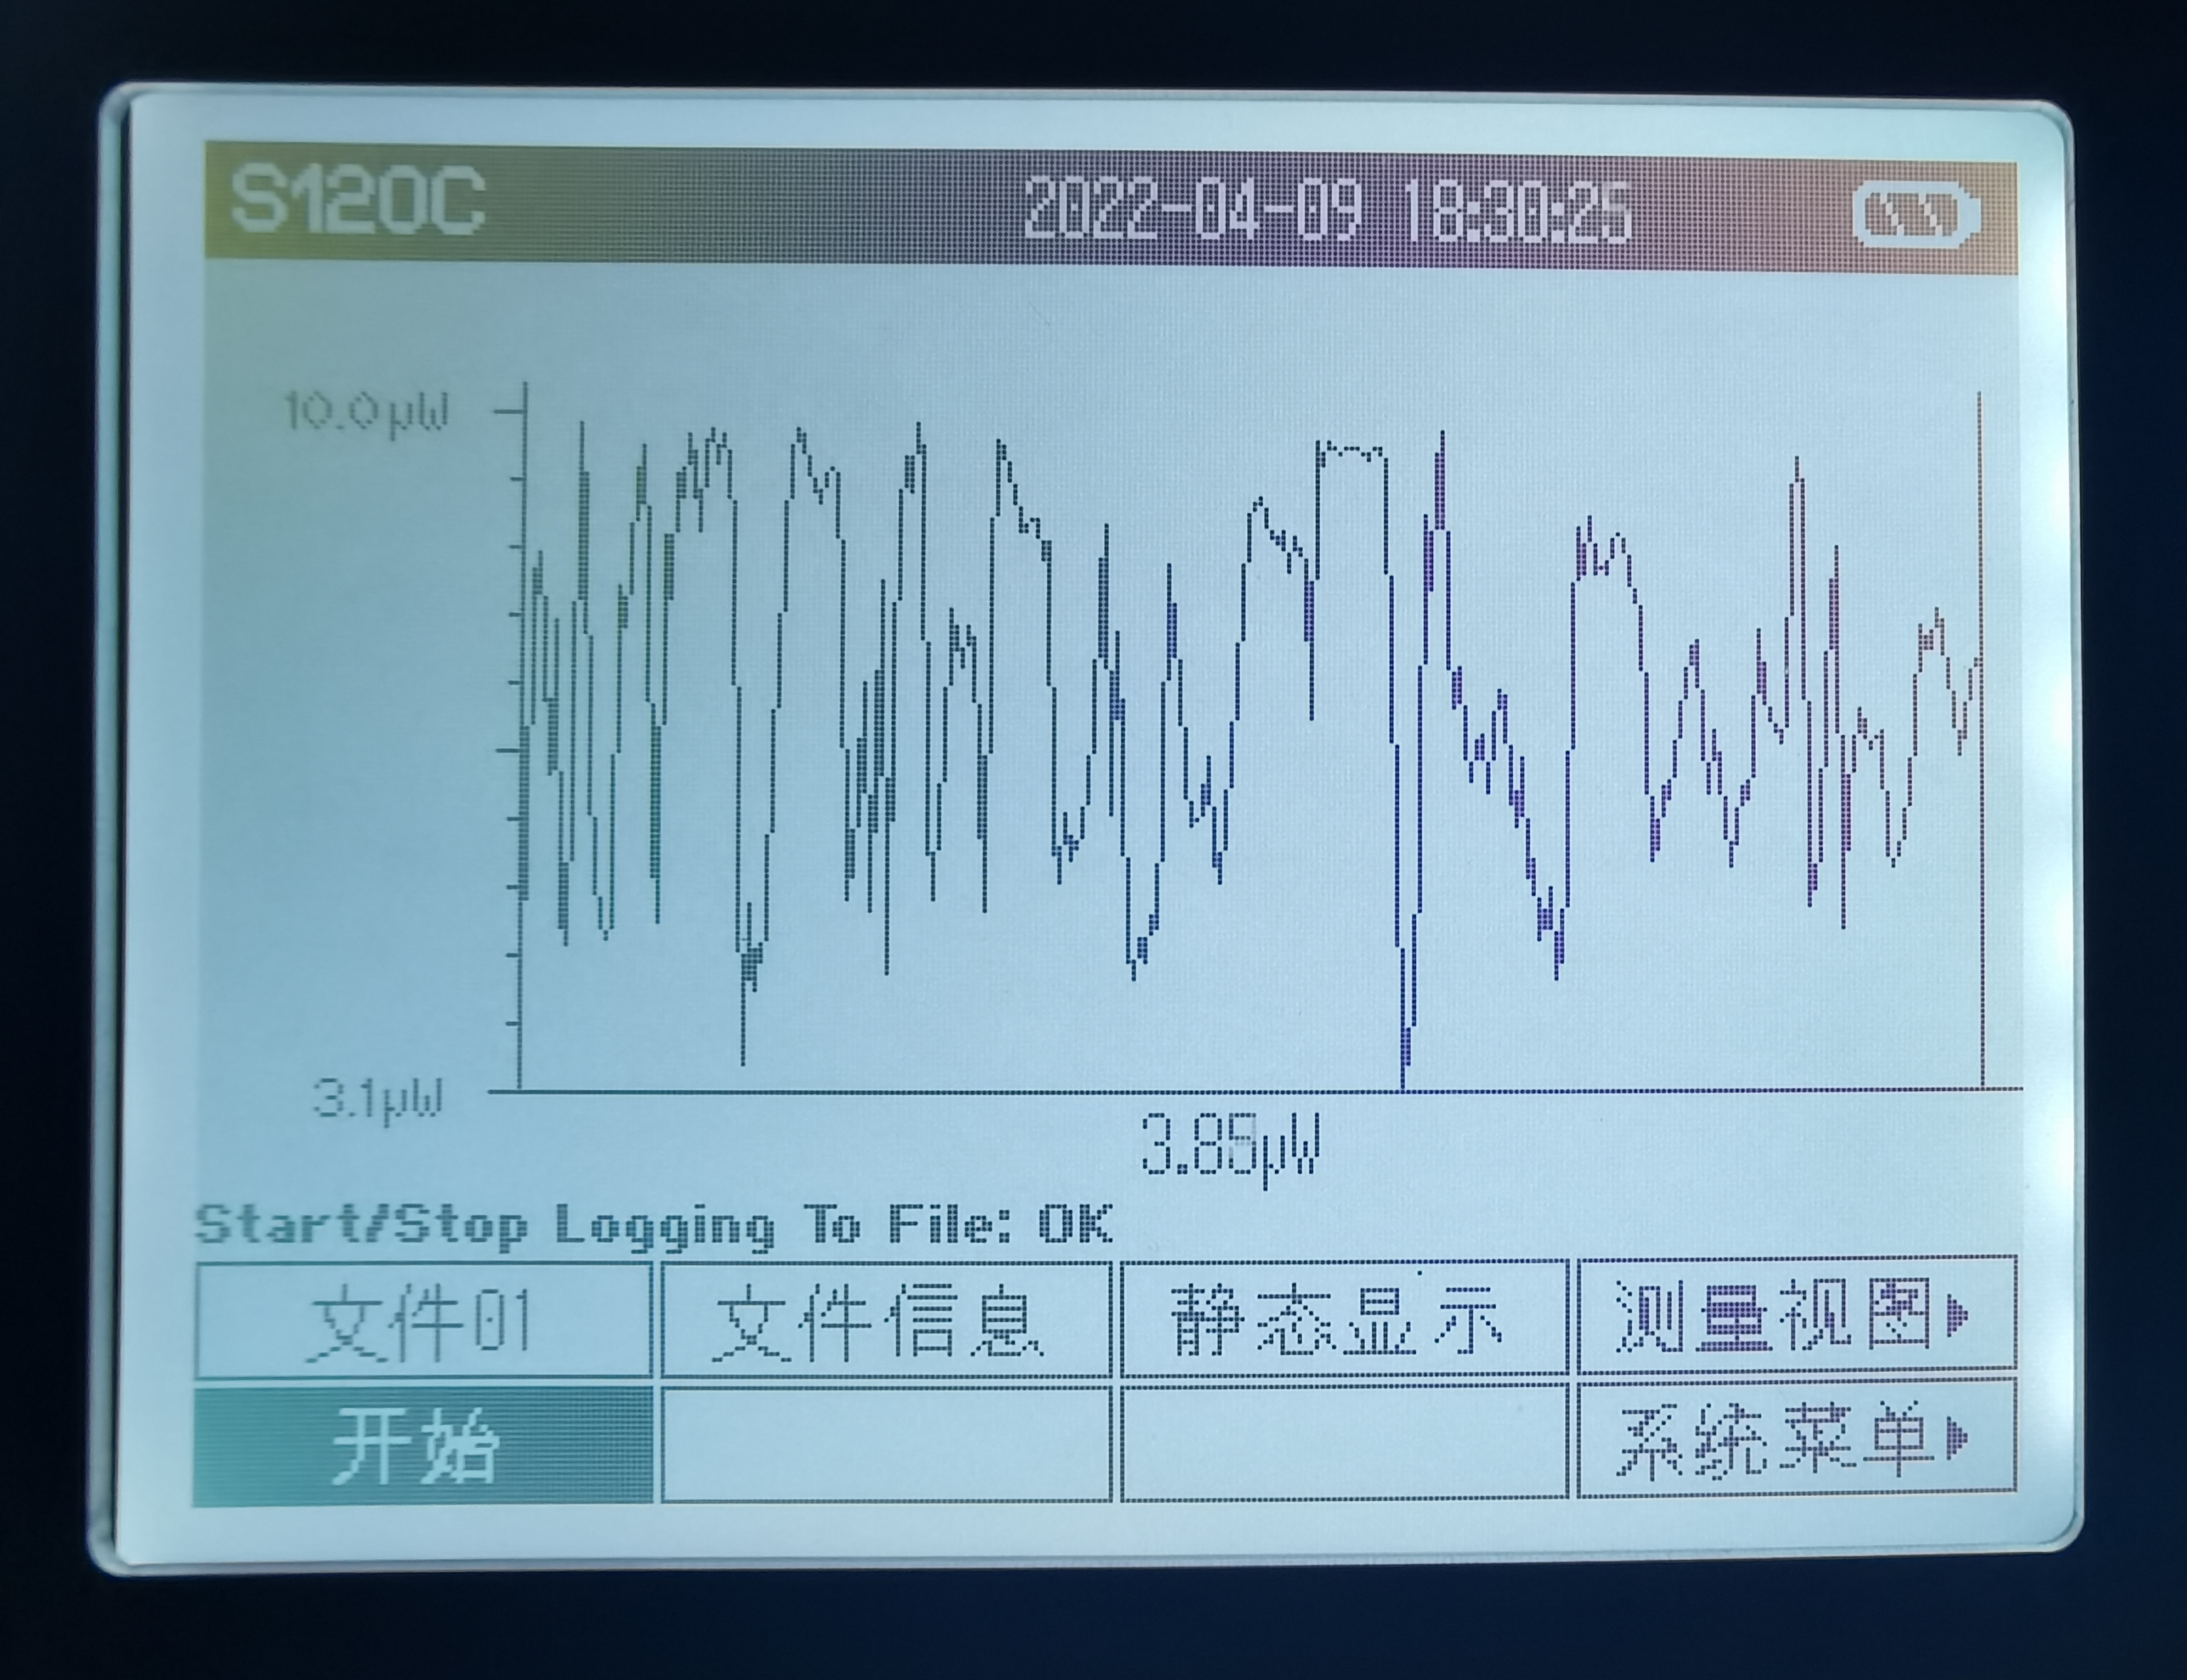
\includegraphics[width=0.5\textwidth]{img//pr.jpg}%调节这里的图片宽度
	\label{fig:10}
\end{figure}
答:(a)和(d)能平衡,(b)和(c)不能。

根据交流电桥的平衡条件可知,电桥四个桥臂的阻抗中必须至少要有两个能够调节,并且$\frac{|Z_1|}{|Z_2|}=\frac{|Z_3|}{|Z_4|}$和$\varphi_1-\varphi_2=\varphi_3-\varphi_4$同时成立才能使电桥
达到平衡状态。如果相邻两臂为纯电阻,则其余两臂必须同时为电感或者电容,因此(b)(d)中(d) 可以,(b)不行;如果相对两臂为纯电阻,则其余两臂必须分别为电感和电容,因此(a)和
(c)中,(a)可以,(c)不行。




\clearpage
	\subsection*{【附录】}
	\subsubsection*{实验器材}
	\begin{figure}[!h]
		\centering
		\includegraphics[width=0.7\textwidth]{img//device.jpg}
			%textwidth:正文宽度。双栏,则将两栏正文宽度相加。
		\label{fig:device}
	\end{figure}


\footnotetext[1]{{Supported and taught by Luyoutang, School of Physics, Sun Yat-sen University}}
\footnotetext[2]{{Corresponding author. E-mail:\url{xxxx@mail2.sysu.edu.cn}}}
%%end--------------------英文摘要------------------------%%


\end{document}
